%-----------------------------------------------------------------------------%
\chapter{\babTiga} \label{chap:metode_penelitian}
%-----------------------------------------------------------------------------%

%-----------------------------------------------------------------------------%
\section{Metode Penelitian}
%-----------------------------------------------------------------------------%
Penelitian tesis ini memanfaatkan dasar teori dependensi yang menjadi ancangan untuk kerangka teori dan metode penelitian. Semua temuan yang dipaparkan dalam penelitian ini didasarkan pada korpus data yang terkumpul dan keterkaitannya terhadap teori yang dibahas. Korpus bahasa Indonesia ragam tulis dan lisan diolah dan dianalisis dengan ancangan yang memadukan pendekatan analisis linguistik kuantitatif dan kualitatif. Langkah-langkah dalam penelitian yang dijelaskan dalam bab ini melibatkan (a) penjelasan mengenai sumber data dan pengumpulan data menjadi dua korpus utama, (b) pengolahan data yang mencakup tahap penguraian kalimat berdasarkan dependensi, anotasi Panjang Dependensi (DL) dan Rata-rata Jarak Dependensi (MDD) terhadap semua ujaran di dalam korpus, seleksi dan klasifikasi data tersebut untuk keperluan analisis, serta (c) teknik-teknik analisis data untuk pemaparan temuan terkait Pengurangan Panjang Dependensi (DLM) dan Pengurangan Jarak Dependensi (DDM) antarkonstituen secara kuantitatif dan analisis kualitatif untuk melihat struktur ujaran-ujaran berdasarkan temuan tersebut, pengaruh panjang kalimat terhadap struktur dependensi, serta perubahan valensi akar verbal.

%-----------------------------------------------------------------------------%
\section{Sumber Data}
%-----------------------------------------------------------------------------%

Merujuk pada pokok permasalahan penelitian ini yang menitikberatkan pada efisiensi ujaran dipandang dari segi dependensi, teks yang digunakan dalam kedua korpus data difokuskan kepada satu aliran, yaitu teks informatif. Pemilihan satu aliran teks ini didasarkan pada pertimbangan untuk menyeimbangkan kuantitas dan kualitas data sehingga analisis tidak melebar akibat perbedaan aliran teks. Sebelumnya, \cite{miller2011critical} melihat adanya perbedaan kerumitan sintaktis dalam teks informatif itu sendiri, seperti halnya media cetak formal akan lebih kompleks dibandingkan dengan artikel tabloid. Hal ini menunjukkan bahwa data penelitian linguistik terkait dependensi dapat fokus kepada salah satu aliran teks (informatif atau imajinatif) dan tetap mendapatkan gambaran keragaman pola yang ada di dalamnya. Penelitian-penelitian terdahulu yang menggunakan dasar teori dependensi dalam konteks bahasa Indonesia menggunakan korpus data hanya mencakup data ragam tulis dari berbagai jenis media seperti jurnalistik, blog, artkel penelitian, dan media sosial sehingga variabel aliran teks tidak menjadi pertimbangan. Pemilahan korpus data tersebut dilakukan dengan dasar keragaman serta kuantitas data untuk mendapatkan gambaran luas pada bahasa Indonesia ragam tulis (\citealp{kamayani2011dependency, green2012indonesian, irmawati2015dependency, futrell2015large}). 

\cite{wang2017effects} menemukan bahwa teks imajinatif seperti novel, cerita pendek, dan karya literatur lainnya cenderung memiliki jarak dependensi yang lebih jauh dibandingkan dengan teks informatif. Sehingga, untuk melihat penekanan dalam efisiensi ujaran dan kaitanya dengan struktur dependensi, aliran teks lebih tepat untuk digunakan dalam penelitian ini. Saat ini, teks informatif tidak hanya hadir dalam media jurnalistik formal tetapi juga dalam blog dan sosial media dengan bahasa tidak baku atau sehari-hari. Namun, sumber daya teknologi untuk mengolah data bahasa non-formal tersebut masih sangat kurang memadai sehingga tidak memungkinkan peneliti untuk melakukan penelitian skala besar \citep{green2012indonesian}. Oleh karena itu, penelitian tesis ini memfokuskan pada data jurnalistik bahasa Indonesia mencakup ragam tulis dan lisan karena memiliki kaidah yang cukup formal untuk dapat dipadankan dibandingkan dengan aliran fiksi yang kaidahnya terlalu bebas. 

%-----------------------------------------------------------------------------%
\subsection{Data Jurnalistik Ragam Tulis}
%-----------------------------------------------------------------------------%
Salah satu cara dalam pengumpulan data untuk korpus jurnalistik ragam tulis ini bekerjasama dengan perusahaan Indonesia bernama Dattabot yang salah satu ruang lingkup kerjanya bergerak di bidang media monitoring. Korpus ragam tulis ini mencakup dokumentasi data jurnalistik dari berbagai media cetak (\pic~\ref{fig:contoh-tulis-mentah}) dengan kurun waktu publikasi dari tahun 2008 hingga 2018. Teks dalam korpus data ragam tulis ini mencakup total 19.530 ujaran atau kalimat yang secara keseluruhan mengandung total 270.409 konstituen. Pemilahan data teks untuk dimasukkan ke dalam korpus penelitian tesis ini dilakukan secara acak dari korpus yang lebih besar milik Dattabot dengan kriteria sebagai berikut:

\begin{itemize}
	\item Jenis media cetak mencakup artikel daring (\textit{online}), surat kabar, majalah, dan tabloid
	\item Topik mencakup berita kriminal, politik, bencana, lalu lintas, hiburan/budaya, pendidikan, teknologi, olahraga, bisnis/keuangan, dan umum
\end{itemize}

\begin{figure}
	\centering 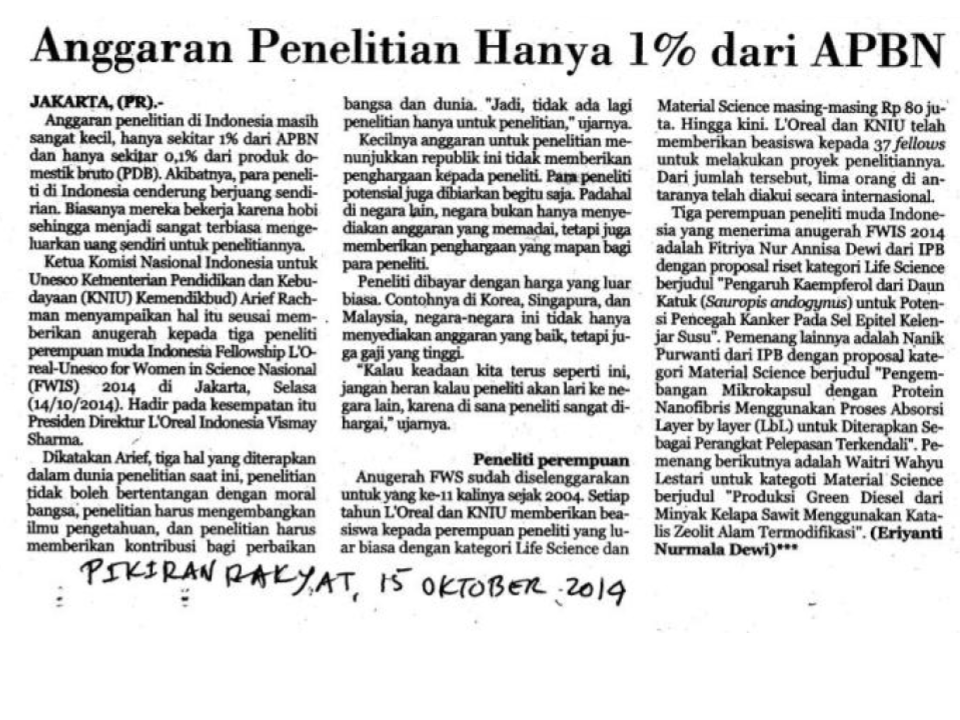
\includegraphics[width=1
	\textwidth] {pics/contoh-tulis-mentah.png} \caption{Contoh data mentah ragam tulis} 
\label{fig:contoh-tulis-mentah} 
\end{figure}

%-----------------------------------------------------------------------------%
\subsection{Data Jurnalistik Ragam Lisan}
%-----------------------------------------------------------------------------%
Penelitian ini memanfaatkan juga dokumentasi data jurnalistik berupa rekaman laporan berita dan wawancara dengan narasumber dengan waktu rekaman dari tahun 2010 hingga 2018. Pengumpulan data ragam lisan dilakukan dengan bantuan para jurnalis dari berbagai media dan daerah di Indonesia yang mengunggah rekaman secara \textit{online} dan video jurnalistik \textit{online} yang ditranskripsi. Teks dalam korpus data ragam lisan ini mencakup total 10.219 ujaran atau kalimat yang secara keseluruhan mengandung total 108.208 konstituen. Pemilahan data ragam lisan untuk dimasukkan ke dalam korpus berdasarkan kriteria sebagai berikut:

\begin{itemize}
	\item Jenis media untuk para jurnalis mencakup televisi, radio, surat kabar, majalah dan tabloid
	\item Topik berita kriminal, politik, bencana, lalu lintas, hiburan/budaya, pendidikan, teknologi, olahraga, bisnis/keuangan, dan umum
	\item Isi rekaman berupa laporan berita atau wawancara dengan narasumber
\end{itemize}

Pengumpulan korpus data ragam lisan memakan waktu lebih lama dibandingkan korpus data ragam tulis karena harus melalui beberapa tahap sebelum dapat diolah pada langkah penelitian selanjutnya. Tahap pertama yang dilakukan untuk persiapan data ragam ilisan adalah proses verifikasi terhadap isi rekaman untuk memastikan tidak lebih dari 10\% isi rekaman yang bersifat pembacaan naskah. Proses persiapan awal ini menjadi perhatian penting untuk mendapatkan kualitas data korpus yang mendekati murni lisan. Tahap kedua dalam persiapan korpus data jurnalistik ragam lisan seperti pada \pic~\ref{fig:contoh-transkripsi-lisan} adalah transkripsi rekaman audio menjadi teks tulisan dengan metode komputasional yang kemudian diverifikasi secara manual agar dapat dianalisis dengan metode serupa seperti yang dilakukan terhadap data ragam tulis. 

\begin{figure}
	\centering 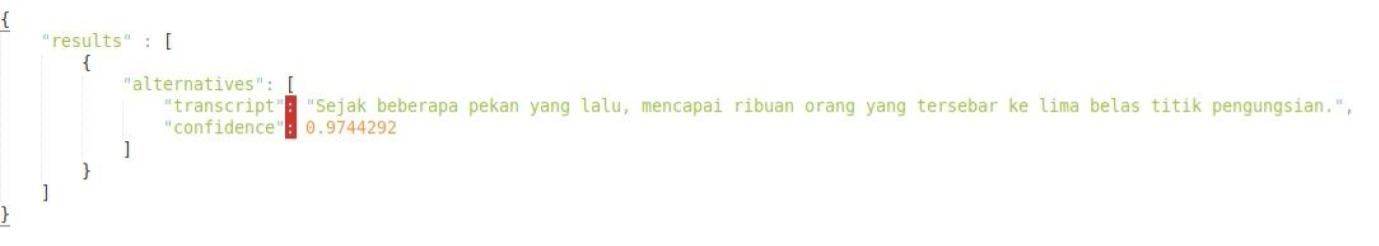
\includegraphics[width=1
	\textwidth] {pics/contoh-transkripsi-lisan.png} 
	\caption{Contoh hasil transkripsi data ragam lisan} 
	\label{fig:contoh-transkripsi-lisan} 
\end{figure}

Tahap terakhir dari persiapan korpus data ragam lisan adalah eliminasi ujaran-ujaran yang tidak selesai agar tidak mengganggu proses pengolahan data. Hal ini dilakukan karena keterbatasan metode penguraian kalimat yang masih belum bisa menguraikan ujaran yang tidak selesai. Dengan proses ini maka seluruh teks dalam data ragam lisan berisi ujaran utuh dan lebih dapat disandingkan dengan data ragam tulis dalam analisisnya.

%-----------------------------------------------------------------------------%
\section{Pengolahan Data}
%-----------------------------------------------------------------------------%

Penelitian ini merupakan penelitian yang bersifat sinkronis terhadap data jurnalistik termutakhir baik untuk ragam tulis maupun lisan. Tujuan utama penelitian ini adalah mengeksplorasi adanya indikasi efisiensi ujaran dan memaparkan strategi-strategi pembentukan struktur ujaran pada kedua ragam. Oleh karena itu, penelitian ini tidak memfokuskan pada leksikon dan konteksnya seperti pada pendekatan linguistik korpus secara umum. Variasi topik dalam pengumpulan data dilakukan untuk memastikan keragaman dalam satu aliran teks tersebut terjaga agar memberikan gambaran dependensi yang tidak terkait topik. Hal ini juga dilakukan untuk mempermudah proses pengolahan data yang mencakup beberapa tahap komputasi.

%-----------------------------------------------------------------------------%
\subsection{Perangkat Pengolahan Data}
%-----------------------------------------------------------------------------%
Data jurnalistik ragam tulis yang diterima dari hasil kerja sama dengan perusahaan media monitoring Dattabot berbentuk teks elektronik hasil pemindaian media cetak dengan pendekatan komputasional \textit{Optical Character Recognition} (OCR). Sedangkan, data jurnalistik ragam lisan berupa rekaman audio yang diolah terlebih dahulu dalam salah satu tahap persiapan data menggunakan metode komputasional dengan bantuan Google Speech API dan diverifikasi kembali secara manual. Tahap penguraian kalimat memanfaatkan UDPipe \citep{udpipe2017} yang merupakan sebuah kerangka kerja yang dapat dilatih ulang untuk pengkategorian konstituen ujaran (\textit{token}), penguraian lemma, dan penguraian kalimat. Kerangka kerja UDPipe digunakan sebagai langkah penguraian kalimat komputasional dan dijalankan sebagai paket CRAN pihak ketiga UDPipe versi 0.5 \cite{udpipe2017manual} pada bahasa pemrograman R (versi 3.3.3) \citep{r2017project}. 

Umumnya, kerangka kerja atau pendekatan penguraian kalimat dalam ranah linguistik komputasional memanfaatkan teori konstituensi sebagai dasar teori dan pengembangannya sehingga menghasilkan uraian kalimat berdasarkan struktur frasanya. Kerangka kerja penguraian kalimat UDPipe menggunakan dasar diagram pohon dependensi Universal Dependencies 2.0 \citep{nivre2017universal} dengan memadukan lemma dan fitur morfologis lainnya dari kerangka kerja MorphInd yang kontekstual terhadap data bahasa Indonesia \citep{larasati2011indonesian}. Kerangka kerja penguraian kalimat berdasarkan dependensi saat ini masih terus dikembangkan secara intensif sehingga masih memiliki kekurangan dalam aspek menangani keambiguitasan makna konstituen, bentuk bahasa informal, dan masalah ujaran nyata lainnya. Kekurangan ini menuntut tahapan verifikasi manual untuk memastikan kualitas data. Meskipun begitu, hasil uji model penguraian kalimat terhadap bahasa Indonesia memiliki akurasi 74,3\%-80,6\% \citep{udpipe:2017}. Setelah melalui proses penguraian kalimat, seluruh tahapan-tahapan berikutnya yang mencakup anotasi nilai DL dan MDD, seleksi dan klasifikasi data, analisis teks, pemaparan pola DL dan MDD, serta uji signifikansi memanfaatkan bahasa pemrograman R (versi 3.3.3) \citep{r2017project} dan Python (versi 3.6.3) (Python Core Team, 2017).

%-----------------------------------------------------------------------------%
\subsection{Penguraian Kalimat}
%-----------------------------------------------------------------------------%
Prinsip mendasar dalam menguraikan tautan dependensi secara sintaktis dapat dilihat pada \pic~\ref{fig:tautandependensi} (\citealp{tesniere1959elements, hudson1984word, liu2008dependency, liu2017dependency}). Secara mendasar, tautan dependensi ini merupakan tautan yang bersifat asimetris dan biner antara dua unit linguistik \citep{tesniere1959elements}. Tautan dependensi yang terbentuk antara dua unit linguistik atau dua konstituen tersebut direpresentasikan oleh panah yang mengarah dari pengendali yang merupakan akar atau induk ke arah subordinatnya yang merupakan konstituen terikat\footnote{Apabila konstituen terikat mengikat konstituen terikat lain, maka subordinat dapat merupakan induk.}. Tautan dependensi yang terbentuk berbeda-beda tergantung dari relasi antara kedua konstituen, sehingga memerlukan anotasi tipe dependensi agar dapat diidentifikasi. Pada \pic~\ref{fig:tautandependensi}, tipe dependensi ini dianotasikan di atas tautan dependensi. Seluruh proses ini dilakukan dengan metode komputasional dengan bantuan UDPipe \citep{udpipe2017} dengan dasar kumpulan diagram pohon dependensi Universal Dependencies 2.0 \citep{nivre2017universal} yang kemudian dikoreksi secara manual.

\begin{figure}
	\centering 
\includegraphics[width=0.6
	\textwidth] {pics/tautandependensi.png} \caption{Elemen-elemen dari tautan dependensi} 
\label{fig:tautandependensi} \end{figure}

Penguraian kalimat merupakan tahapan komputasional utama dalam tahap pengolahan data penelitian sesuai dengan teori yang dijabarkan pada bab sebelumnya. Pada penelitian ini, penguraian kalimat UDPipe mengadopsi Indonesian UD. Indonesian UD berisi kumpulan diagram pohon dependensi hasil konversi Universal Dependencies 2.0 \citep{nivre2017universal} yang dikondisikan khusus untuk Bahasa Indonesia. Anotasi tipe dependensi seperti pada contoh \pic~\ref{fig:contohtulis} dan \pic~\ref{fig:contohlisan} menyesuaikan dengan daftar anotasi dalam panduan dependensi milik Stanford Parser \citep{de2008stanford}. \pic~\ref{fig:contohtulis} dan \pic~\ref{fig:contohlisan} merupakan hasil visualisasi mandiri untuk memudahkan pemahaman tautan dependensi berdasarkan hasil penguraian dengan bantuan UDPipe. Kedua ujaran tersebut diambil dari korpus data ragam tulis dan lisan yang telah dibangun. UDPipe tidak memiliki masalah dalam pengolahan kedua contoh data dari ragam tulis dan lisan ini meskipun kedua contoh data tidak memiliki aktor pelaku. Namun, pada beberapa ujaran yang lain, UDPipe masih memiliki masalah dalam menguraikannya sehingga diperlukan tahapan verifikasi manual untuk memastikan kualitas data. Skema anotasi yang dihasilkan berdasarkan tahap penguraian kalimat ini bersifat lintas bahasa yang awalnya dikembangkan untuk Bahasa Inggris kemudian berkembang menjadi 60 bahasa, termasuk Bahasa Indonesia (\citealp{de2008stanford, nivre2017universal}). 

\begin{figure}
	\centering 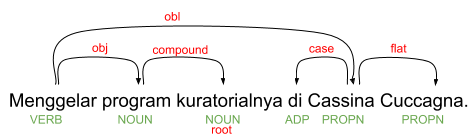
\includegraphics[width=0.5
	\textwidth] {pics/contohtulis.png} \caption{Contoh hasil penguraian kalimat untuk data ragam tulis} 
\label{fig:contohtulis} \end{figure}

\begin{figure}
	\centering 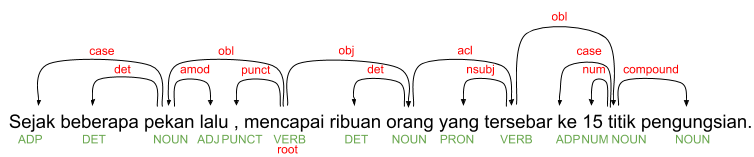
\includegraphics[width=0.85
	\textwidth] {pics/contohlisan.png} \caption{Contoh hasil penguraian kalimat untuk ragam lisan} 
\label{fig:contohlisan} \end{figure}

Kontekstualisasi treebank dependensi yang bersifat lintas bahasa dilakukan dengan melibatkan MorphInd \citep{larasati2011indonesian}, sebuah pendekatan morfologis dan penguraian lemma untuk pengolahan bahasa. MorphInd memiliki aturan morfofonemik dan morfosintaktis untuk menganalisis kata-kata Bahasa Indonesia yang mengalami infleksi dan derivasi. Hasil olahan MorphInd mengintegrasikan penandaan morfologis pada sebuah kata seperti pada \pic~\ref{fig:morphind_schema}.

\begin{figure}
	\centering 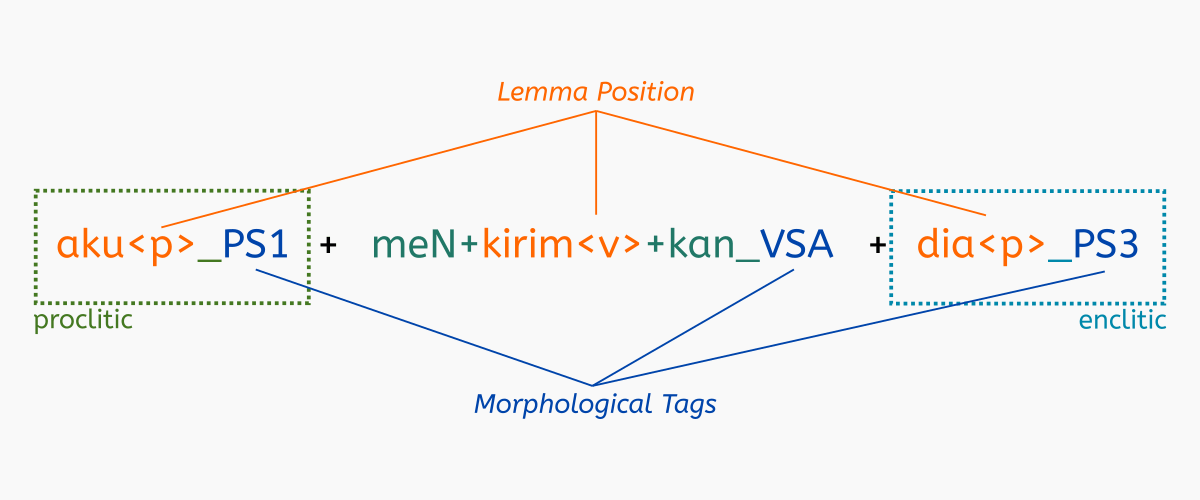
\includegraphics[width=1
	\textwidth] {pics/morphind_schema.png} \caption{Contoh hasil ekstraksi lemma dengan memanfaatkan MorphInd (Larasati, Kubo?, & Zeman, 2011) } 
\label{fig:morphind_schema} 
\end{figure}

Penelitian ini mengikuti panduan dependensi milik Stanford Parser \citep{de2008stanford} yang mengikutsertakan tanda baca yang terlibat dalam kalimat. Penelitian ini tidak mengikutsertakan tanda baca pada akhir kalimat dalam penghitungan jarak dependensi karena tanda baca di akhir kalimat tidak memberikan pengaruh terhadap jumlah tautan dependensi yang terjadi dalam sebuah ujaran. Namun, tanda baca pada akhir kalimat tetap diperhatikan untuk analisis karena dapat menjadi indikasi perbedaan jenis kalimat maka yang mendorong perbedaan perilaku tautan dependensi yang ada. Tanda baca koma yang mewakili jeda atau \textit{pause} dilibatkan dalam proses penguraian kalimat karena memiliki peran sintaktis yang harus diperhitungkan. Dependensi tipe Stanford \citep{de2008stanford} umumnya memilih konstituen kata penuh dibandingkan dengan konstituen kata tugas sebagai induk sintaktis, kecuali untuk konstruksi kopula (tergantung kasus) dan frasa adposisi seperti pada diagram pohon dependensi bahasa Indonesia dalam Universal Dependencies 2.0 \citep{nivre2017universal}. Berikut adalah deskripsi yang membandingkan kedua jenis konstituen kata tersebut berdasarkan Kamus Linguistik \citep{kridalaksana2008kamus}:

\begin{itemize}
	\item \textbf{kata penuh} (\textit{content word} atau \textit{full word}) merupakan kata yang mempunyai makna leksikal yang bebas seperti 'rumah', 'angin', 'orang', dan lain sebagainya.
	\item \textbf{kata fungsi} (\textit{function word}) merupakan kata yang terutama menyatakan hubungan gramatikal yang tidak dapat bergabung dengan afiks, dan tidak mengandung makna antara lain adalah preposisi, konjungsi, artikel, dan pronomina.
\end{itemize}

 \tab~\ref{tab:tipe_anotasi} berikut berisi anotasi tipe dependensi dan deskripsi singkat berdasarkan Universal Dependencies 2.0 \citep{nivre2017universal} yang diadopsi dari panduan dependensi milik Stanford Parser \citep{de2008stanford}.

\begin{center}
\begin{small}
\begin{longtable}{| p{.20\textwidth} | p{.80\textwidth} |} 
\caption{Tipe anotasi dan deskripsi singkat berdasarkan Universal Dependencies 2.0 \citep{nivre2006maltparser}} \label{tab:tipe_anotasi}
    \hline
Anotasi & Deskripsi Tipe Anotasi \\ \hline
ROOT & Induk pohon dependensi \\ \hline
acomp & Pelengkap ajektival, termasuk pelengkap predikatif \\ \hline
adp / adpos & Adposisi yang dianalisis sebagai konstituen yang bergantung pada nomina \\ \hline
adpcomp / pcomp & Pelengkap klausal dari adposisi \\ \hline
adpmod / prep / postp & Pewatas adposisi \\ \hline
adpobj / pobj & Pelengkap nominal dari adposisi \\ \hline
advcl & Pewatas klausa adverbial \\ \hline
advmod & Pewatas adverbial \\ \hline
amod & Pewatas apposisi \\ \hline
attr & Pelengkap predikatif nominal (bergantung pada verba kopula) \\ \hline
aux & Verba bantu (bergantung pada verba induk) \\ \hline
auxpass & Verba bantu pada konstruksi pasif \\ \hline
cc & Konjungsi koordinatif (bergantung pada konjungsi) \\ \hline
ccomp & Pelengkap klausal \\ \hline
ccompmod & Pewatas kompositum (bagian kompositum yang bukan induk) \\ \hline
conj & Konjungsi \\ \hline
cop & Verba kopula \\ \hline
csubj & Subyek klausal \\ \hline
csubjpass & Subyek klausal dalam konstruksi pasif \\ \hline
dep & Konstituen terikat yang tidak terklasifikasi \\ \hline
det & Determinator \\ \hline
dobj & Obyek langsung \\ \hline
expl & Subyek (seruan) \\ \hline
infmod & Pewatas infinitif \\ \hline
iobj & Obyek tidak langsung \\ \hline
mark & Konjungsi subordinat dan ekspresi setara \\ \hline
mwe & Ekspresi multi kata, termasuk nama dengan multi kata \\ \hline
neg & Negasi \\ \hline
nmod / nommod / nommod-own / npadvmod & Pewatas nominal \\ \hline
nsubj & Subyek nominal \\ \hline
nsubjpass & Subyek nominal dalam konstruksi pasif \\ \hline
num & Numeralia \\ \hline
p / punct & Tanda baca \\ \hline
parataxis & Struktur serupa klausa yang bergantung pada klausa sebelumnya \\ \hline
partmod & Pewatas partisipel \\ \hline
poss & Pewatas posesif (atau genitif) \\ \hline
prt & Partikel verba \\ \hline
rcmod & Pewatas klausa relatif \\ \hline
rel & Pronomina atau adverbia relatif dengan fungsi yang tidak terklasifikasi \\ \hline
vmod & Pewatas verbal \\ \hline
xcomp & Pelengkap infinit serupa klausa \\ \hline
    \hline
  \end{longtable}
\end{small}
\end{center}

\todo{tambahin penjelasan mengenai hubungan klausa}

%-----------------------------------------------------------------------------%
\subsection{Anotasi Panjang Dependensi (DL) dan Rata-rata Jarak Dependensi (MDD) Antarkonstituen}
%-----------------------------------------------------------------------------%
Setelah kedua korpus data diuraikan dengan pendekatan komputasional, tabel hasil penguraian data diberikan anotasi kolom tambahan berisi anotasi nilai hasil penghitungan DL dan MDD. Anotasi ini dilakukan tidak hanya pada masing-masing ujaran, namun juga pada masing-masing relasi yang ada dalam ujaran tersebut. Penghitungan untuk mendapatkan nilai DL dan MDD tergabung menjadi dua tahapan yang berkelanjutan karena untuk mendapatkan nilai MDD, dibutuhkan nilai DL terlebih dahulu. Langkah pertama dalam tahapan anotasi nilai DL dan MDD ini adalah menguraikan ujaran di dalam kedua korpus sesuai prinsip penghitungan panjang dan jarak dependensi. Seluruh ujaran di dalam kedua korpus diperlakukan sebagai deretan konstituen $W1...Wi...Wn$. Jarak dependensi (DD) antara konstituen $Wa$ dengan konstituen $Wb$ dapat dihitung dari selisih keduanya (\citealp{liu2008dependency, liu2017dependency, futrell2015large}) sehingga konstituen-konstituen yang bersebelahan atau berdampingan memiliki jarak dependensi sejumlah 1. Untuk memperhitungkan arah dependensi dalam penghitungan ini, selisih antara kedua konstituen perlu dibedakan menyesuaikan dengan arah panah tautan dependensi tersebut:
\begin{itemize}
\item Apabila $a$ merupakan induk dan posisinya sebelum $b$ yang merupakan konstituen terikatnya, maka anotasi yang diberikan bernilai \textbf{positif}.
\item Sedangkan, apabila $a$ merupakan induk dan posisinya berada setelah $b$ yang merupakan konstituen terikatnya, maka anotasi yang diberikan bernilai \textbf{negatif}. 
\end{itemize}
Dalam melihat kecenderungan Pengurangan Panjang Dependensi (DLM), nilai yang dianalisis adalah nilai Panjang Dependensi atau DL. DL didapatkan dengan menjumlahkan semua nilai DD dalam satu ujaran (\citealp{gildea2010grammars, futrell2015large}) dengan rumus sebagai berikut: 

\noindent \begin{align}\label{eq:bola}
	\displaystyle\sum_{i=1}^{n-1} |DD_i|
\end{align}

Penelitian ini juga melihat kecenderungan Pengurangan Jarak Dependensi (DDM) dengan menganalisis nilai Rata-rata Jarak Dependensi (MDD) (\citealp{liu2008dependency, liu2017dependency}) dengan rumus sebagai berikut:

\noindent \begin{align}\label{eq:bola}
	\frac{1}{n-1} \displaystyle\sum_{i=1}^{n-1} |DD_i|
\end{align}

Pada kedua rumus tersebut, $n$ adalah jumlah konstituen di sebuah kelimat. $DDi$ adalah jarak dependensi dengan tautan sejumlah $i$. Dalam kata lain, MDD didapatkan dari nilai DL (yang merupakan jumlah dari nilai absolut DD dalam sebuah ujaran) dibagi dengan jumlah tautan dependensi dalam ujaran tersebut. Berdasarkan dua ujaran contoh dari data ragam tulis (\pic~\ref{fig:contohtulis}) dan ragam lisan (\pic~\ref{fig:contohlisan}) di atas, maka anotasi nilai DL dan MDD digambarkan pada visualisasi mandiri seperti pada \pic~\ref{fig:contohtulis_DLMDD} dan \pic~\ref{fig:contohlisan_DLMDD}.

\begin{figure}
	\centering 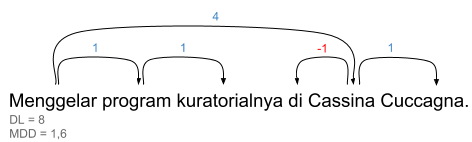
\includegraphics[width=0.5
	\textwidth] {pics/contohtulis_DLMDD.png} \caption{Contoh hasil olahan penghitungan jarak antarkata data ragam tulis} 
\label{fig:contohtulis_DLMDD} 
\end{figure}

\begin{figure}
	\centering 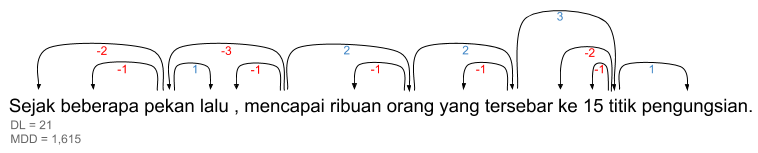
\includegraphics[width=0.85
	\textwidth] {pics/contohlisan_DLMDD.png} \caption{Contoh hasil olahan penghitungan jarak antarkata data ragam lisan} 
\label{fig:contohlisan_DLMDD} 
\end{figure}

Pada contoh di atas, kalimat dari ragam tulis pada \pic~\ref{fig:contohtulis_DLMDD} memiliki nilai DL (atau total nilai DD dalam ujaran tersebut) sejumlah 8 dan jumlah tautan dependensi sebanyak 5 sehingga nilai MDD yang didapat adalah 1,6. Hal ini berarti rata-rata jarak antara dua konstituen dalam ujaran tersebut adalah sejauh 1,6 konstituen. Ujaran ini memiliki empat tautan positif (induk sebelum konstituen terikat) dan satu tautan negatif (induk setelah konstituen terikat), yaitu pada relasi antara 'Cassina' dan 'di'. Karena jumlah konstituen dalam ujaran ini di bawah 10 konstituen, maka kalimat ragam tulis ini masuk ke dalam klasifikasi kalimat pendek. Sedangkan, kalimat dari ragam lisan \pic~\ref{fig:contohlisan_DLMDD} memiliki nilai DL sejumlah 21 dan jumlah tautan dependensi sebanyak 13 sehingga nilai MDD yang didapat adalah 1.615 yang berarti rata-rata jarak antara dua konstituen dalam ujaran tersebut adalah sejauh 1,615 konstituen. Kalimat ragam lisan tersebut masuk ke dalam klasifikasi data ragam lisan dengan panjang kalimat di atas 20 konstituen atau klasifikasi kalimat panjang. Berbeda dengan contoh ragam tulis, ujaran ini memperlihatkan jumlah tautan negatif yang lebih banyak dibandingkan tautan positif.

%-----------------------------------------------------------------------------%
\subsection{Klasifikasi Data}
%-----------------------------------------------------------------------------%
Salah satu penjabaran pokok permasalahan menitikberatkan pada pengaruh panjang kalimat dalam penyusunan struktur ujaran atau kalimat yang efisien dalam bahasa Indonesia dipandang dari segi dependensi. Tidak hanya dari segi panjang kalimat, penelitian ini juga menitikberatkan pada perbandingan perilaku dependensi dalam ujaran yang formal dan ujaran yang lebih spontan. Kedua aspek ini diwakili oleh jenis ragam yaitu tulis dan lisan. Berikut adalah kriteria utama untuk tahap klasifikasi terhadap keseluruhan data.

\begin{itemize}
	\item Untuk melihat perbandingan dasar antara ujaran formal dengan ujaran yang lebih spontan, maka data korpus perlu diklasifikasikan menjadi dua, yaitu data ragam tulis dan ragam lisan.
	\item Terkait dengan uraian permasalahan mengenai pengaruh panjang kalimat dalam penyusunan struktur ujaran yang mungkin juga mempengaruhi jarak dan arah dependensi, maka data korpus akan diklasifikasikan menjadi tiga berdasarkan panjang kalimat di bawah 10 konstituen (dikategorikan sebagai kalimat pendek), 11 hingga 20 konstituen (dikategorikan sebagai kalimat menengah), dan di atas 20 koonstituen (dikategorikan sebagai kalimat panjang). Pendekatan ini menindaklanjuti temuan penelitian \cite{oya2011syntactic} serta \cite{jiang2015effects} yang menggunakan klasifikasi serupa. 
\end{itemize}

Kedua poin ini mendasari langkah klasifikasi terhadap kedua korpus data untuk memudahkan proses agregasi data dalam langkah analisis berikutnya (Tabel \ref{tab:tabel_klasifikasi_data}). 

\begin{table}
\begin{center}
  \caption{Klasifikasi data penelitian}\label{tab:tabel_klasifikasi_data}
  \begin{tabular}{ | l | l | l | l |}
    \hline
    Ragam / Panjang kalimat & \textless 10 konstituen & 11 - 20 konstituen & \textgreater 20 konstituen \\ \hline
    Tulis & Tulis \textless 10 konstituen & Tulis 11 - 20 konstituen & Tulis \textgreater 20 konstituen  \\ \hline
    Lisan & Lisan \textless 10 konstituen & Lisan 11 - 20 konstituen & Lisan \textgreater 20 konstituen \\
    \hline
  \end{tabular}
\end{center}
\end{table}

%-----------------------------------------------------------------------------%
\section{Teknik Analisis Data}
%-----------------------------------------------------------------------------%

Serangkaian tahapan analisis data dengan pendekatan kuantitatif dan kualitatif dilakukan untuk mendapatkan gambaran awal mengenai fenomena efisiensi ujaran dalam bahasa Indonesia dipandang dari segi dependensi serta strategi-strategi yang mungkin diterapkan oleh penutur untuk menghasilkan efisiensi tersebut. Sejauh pemahaman saya dari hasil tinjauan terhadap penelitian-penelitian terdahulu, penelitian ini merupakan penelitian pertama yang mencoba untuk memberikan wawasan linguistik terhadap masalah tersebut sehingga beberapa metode-metode analisis yang diterapkan untuk menganalisis hasil olahan data bersifat eksperimental karena mengadopsi pendekatan yang sebelumnya menggunakan data bahasa lain. Tahap analisis ini diawali dengan uji hipotesis fenomena DLM dalam bahasa Indonesia untuk memberikan bukti empiris adanya efisiensi ujaran berdasarkan korpus data yang dikumpulkan. Langkah-langkah selanjutnya menggabungkan ancangan kuantitatif dan kualitatif untuk membedah hasil olahan data sesuai dengan pokok permasalahan penelitian yang diajukan pada Bab 1.

%-----------------------------------------------------------------------------%
\subsection{Percobaan Acak untuk Menguji Hipotesis Efisiensi Ujaran}
%-----------------------------------------------------------------------------%
Sebelum melakukan identifikasi terhadap karakteristik struktur dependensi berdasarkan korpus data yang dikumpulkan, perlu dilakukan uji hipotesis terhadap asumsi adanya efisiensi ujaran dalam bahasa Indonesia dari segi dependensi. Sebelumnya, uji hipotesis efisiensi ujaran dengan melihat nilai DLM pada bahasa Indonesia pernah dilakukan oleh \cite{futrell2015large} secara lintas bahasa. Namun, percobaan yang dilakukan \cite{futrell2015large} menggunakan korpus data yang berbeda, yaitu data ragam tulis dalam berbagai aliran teks seperti artikel penelitian, \textit{blog}, artikel berita, dan data dari media sosial. Penelitian ini mengadopsi pendekatan percobaan acak yang dilakukan oleh \cite{futrell2015large} dan \cite{gildea2010grammars}. \cite{futrell2015large} menyebut algoritma acak ini dengan istilah \textit{Free Word Order Baseline}, sedangkan \cite{gildea2010grammars} menyebut algoritma acak ini dengan istilah \textit{unlabeled Dependency Linearization Algorithm} (\textit{unlabeled} DLA). Secara prinsip, kedua algoritma ini memiliki kesamaan, yaitu kedua algoritma acak tersebut menyusun ulang konstituen-konstituen dalam ujaran tanpa memperhitungkan aturan tata bahasa yang ada. Sebagai contoh, tidak ada konsistensi apakah aktor pelaku mendahului atau berada setelah verba. Perbedaan kedua algoritma ini terletak pada penerapan algoritma tersebut. 

\cite{gildea2010grammars} menggunakan algoritma \textit{unlabeled} DLA untuk mengubah bentuk ujaran hasil observasi $U$ menjadi bentuk ujaran acak baru dengan nilai DL yang paling kecil $Umin$ dalam arti $Umin$ merupakan bentuk paling efisien (dari segi dependensi) dari $U$ dan membandingkan nilai DL yang didapatkan keduanya. Sementara, \cite{futrell2015large} menerapkan algoritma acaknya terhadap $U$ sebanyak 100 kali untuk menghasilkan ujaran dengan nilai-nilai DL baru dari $U1$ hingga $U100$. \cite{futrell2015large} dan \cite{gildea2010grammars}menyebutkan bahwa $Umin$ yang dihasilkan mungkin tidak bersifat gramatikal maupun berterima. Namun, \cite{futrell2015large} juga menyebutkan pengecualian terhadap bahasa Indonesia yang menghasilkan $Umin$ yang sangat mendekati $U$. Langkah-langkah yang dilakukan dalam algoritma acak ini dijabarkan sebagai berikut:
\begin{enumerate}
\item Identifikasi akar dan semua konstituen terikat yang memiliki tautan dependensi langsung terhadap akar tersebut (level simpai pusat).
\item Penyusunan acak terhadap urutan konstituen pada level simpai pusat.
\item Identifikasi konstituen terikat yang merupakan induk terhadap konstituen terikat lain (level simpai cabang).
\item Penyusunan acak terhadap urutan konstituen pada level simpai cabang.
\item Pengulangan proses pada induk di simpai-simpai cabang berikutnya.
\end{enumerate}
Poses tersebut akan menghasilkan $U1$ sehingga diulang sebanyak 100 kali untuk menghasilkan 100 ujaran dengan susunan acak \citep{futrell2015large}. Berdasarkan tinjauan terhadap kedua pendekatan tersebut dan temuan mengenai data bahasa Indonesia yang didapatkan \cite{futrell2015large}, penelitian ini mengadopsi pendekatan algoritma acak yang dilakukan oleh \cite{futrell2015large}.

Analisis terhadap percobaan acak dilakukan juga dengan mempertimbangkan panjang kalimat yang terkontrol (\textit{controlled sentence length}) antara korpus data hasil observasi dan korpus data kalimat acak. Hal ini dilakukan berdasarkan argumen signifikansi dalam menganalisis dengan panjang kalimat terkontrol sempat dikemukakan oleh \cite{ferrer2014risks} dan \cite{jiang2015effects} serta keterbatasan kapasitas komputasi untuk mengolah korpus berskala besar. Oleh karena itu, percobaan ini dilakukan sebanyak enam kali untuk panjang kalimat dengan frekuensi terbanyak pada masing-masing klasifikasi dari setiap ragam. Perbandingan nilai DL dari korpus data hasil observasi dan korpus data hasil percobaan acak kemudian divisualisasikan melalui histogram dari keduanya. Algoritma acak untuk percobaan ini dijalankan pada bahasa pemrograman Python (versi 3.6.3) (Python Core Team, 2017) kemudian dianalisis dan divisualisasikan pada bahasa pemrograman R (versi 3.3.3) \citep{r2017project} dengan menggunakan paket CRAN untuk visualisasi Plotly \citep{sievert2017plotly}).

%-----------------------------------------------------------------------------%
\subsection{Analisis Pengaruh Persebaran Panjang Kalimat Terhadap Efisiensi Ujaran}
%-----------------------------------------------------------------------------%
Sebelum tahap ini, seluruh ujaran dalam kedua korpus data telah melalui penghitungan nilai DL dan MDD dan telah diklasifikasi berdasarkan panjang kalimatnya. Analisis pengaruh persebaran panjang kalimat terhadap efisiensi ujaran mencoba melihat relasi yang terjadi antara panjang kalimat dan nilai DL serta MDD yang didapatkan. Seperti yang dijelaskan sebelumnya, pertimbangan untuk mencari nilai DL dan MDD menitikberatkan pada dua hal yang sedikit berbeda sehingga pada tahap ini, kedua nilai dipaparkan karena diduga mengandung informasi yang berbeda juga. Tahap ini juga memperhitungkan spontanitas ujaran sehingga perbandingan nilai DL dan MDD antara ragam tulis dan lisan penting untuk dianalisis. 

Langkah pertama yang dilakukan adalah membandingkan persebaran frekuensi panjang kalimat secara keseluruhan antara kedua korpus data dan menganalisis perbandingan tersebut untuk melihat adanya kecenderungan terhadap panjang kalimat secara umum. Langkah berikutnya adalah memisahkan korpus data pada setiap ragam menjadi tiga korpus yang lebih kecil sesuai dengan klasifikasi panjang kalimatnya yaitu kalimat pendek (maksimal 10 konstituen), kalimat menengah (11 hingga 20 konstituen), dan kalimat panjang (minimal 21 konstituen). Sehingga, didapatkan enam korpus yang lebih kecil dari kedua ragam ujaran. Kemudian, rata-rata (\textit{mean}) dihitung berdasarkan nilai-nilai DL dan MDD yang didapatkan oleh setiap ujaran dari korpus-korpus tersebut dan dipaparkan sesuai dengan masing-masing klasifikasi. Perbandingan antara nilai-nilai dari masing-masing klasifikasi pada data ragam tulis dengan data ragam lisan dianalisis untuk melihat adanya perbedaan perilaku efisiensi ujaran (DLM dan DDM). Analisis kualitatif dilakukan untuk melihat adanya perbedaan struktur ujaran pada masing-masing klasifikasi atau antara kedua korpus data.

%-----------------------------------------------------------------------------%
\subsection{Analisis Arah Dependensi}
%-----------------------------------------------------------------------------%
Salah satu pertanyaan penelitian menitikberatkan pada jarak dan arah dependensi yang muncul berdasarkan data yang dikumpulkan. Arah dependensi berkaitan dengan hierarki relasi antara induk dan konstituen terikatnya. Seperti yang dijelaskan pada bab sebelumnya dan divisualisasikan pada \pic~\ref{fig:tautandependensi}, relasi antara dua konstituen dihubungkan dengan sebuah tautan yang memiliki panah. Arah panah tersebut merepresentasikan hierarki relasi antara keduanya. Arah panah ke kanan menandakan tautan yang bernilai positif, dan sebaliknya, arah panah ke kiri menandakan tautan yang bernilai negatif. Hal ini dapat dilihat juga pada visualisasi dari dua ujaran contoh yang diambil dari data ragam tulis (\pic~\ref{fig:contohtulis}) dan ragam lisan (\pic~\ref{fig:contohlisan}). Kedua visualisasi ini mengandung nilai-nilai tautan dengan anotasi positif ($+$) dan anotasi negatif ($-$) (yang juga dibedakan oleh warna biru dan merah) untuk memberikan gambaran terhadap perbedaan arah tautan dependensi dalam sebuah ujaran. Sebagai contoh, \pic~\ref{fig:contohtulis} memiliki 4 tautan positif dan 1 tautan negatif, sehingga pada kalimat ini relasi di mana induk direalisasikan sebelum konstituen terikat mendominasi ujaran tersebut. Pada level dependensi utama atau simpai pusat, 'menggelar' memiliki 2 tautan positif terhadap 'program' dan 'Cassina' dan 0 tautan negatif.

Simpai pusat merepresentasikan relasi-relasi utama dalam sebuah ujaran berdasarkan dependensi. Pada kalimat yang lebih kompleks, simpai pusat juga memberikan gambaran terhadap relasi-relasi utama, namun terkadang banyak relasi pada cabang yang tidak terwakili. Oleh karena itu, pemaparan kedua analisis arah dependensi pada relasi-relasi secara keseluruhan dan pada simpai pusat penting untuk disampaikan. Pada tahap anotasi nilai DL, setiap relasi antara dua konstituen dalam sebuah ujaran sudah diberikan anotasi positif maupun negatif. Sehingga, pada tahap ini hanya perlu dilakukan agregasi data terhadap relasi-relasi bernilai positif dan relasi-relasi bernilai negatif. Tahap analisis ini didasarkan pada diskusi mengenai percabangan searah dan percabangan beda arah yang dibahas oleh \cite{temperley2008dependency} dan \cite{dryer1992greenbergian} untuk melihat adanya kecenderungan dalam menerapkan tipe percabangan keduanya.

%-----------------------------------------------------------------------------%
\subsection{Pengamatan Perubahan Valensi Akar Verbal}
%-----------------------------------------------------------------------------%
Tahap analisis ini masih berkaitan erat dengan analisis arah dependensi karena keterkaitan valensi konstituen dalam sebuah ujaran dengan efisiensi ujaran tersebut tidak hanya dapat diamati melalui pengurangan nilai valensi. Sebuah konstituen dapat mempertahankan nilai valensinya tetapi tetap menghasilkan ujaran yang efisien, yaitu dengan mengatur letak konstituen yang diikatnya sehingga menempati posisi yang paling optimal (menghasilkan nilai DL terkecil). Analisis ini saya lakukan untuk melihat tautan dependensi dan hubungan induk dengan konstituen terikat secara lebih dekat terutama terkait kecenderungan penutur dalam menghasilkan ujaran yang efisien. Meskipun penelitian ini tidak menganalisis leksikon, prinsip dasar yang membentuk kemungkinan pola valensi dalam \textit{Probabilistic Valency Pattern} (PVP) \citep{liu2006syntactic} menjadi dasar pengamatan ini. Perlu saya tekankan bahwa \cite{liu2006syntactic} menganggap valensi sebagai kapasitas sebuah konstituen yang memiliki kualitas gabungan (\textit{combinatorial}). Hal ini berarti sebuah konstituen memiliki valensi tertentu dalam arti dapat mengikat konstituen lain, tetapi juga dapat bertindak sebagai konstituen yang diikat oleh induk lain. Penelitian ini mengamati valensi akar verbal pada simpai pusat pada tataran kalimat sehingga tidak ada aspek konstituen tersebut sebagai konstituen yang diikat induk lain karena dalam ujaran atau kalimat tersebut, konstituen yang diamati berada di posisi teratas dari hierarki dependensi.

Karena keterbatasan sumber daya linguistik untuk menganalisis valensi secara menyeluruh, pengamatan ini dilakukan secara manual dengan analisis kualitatif berdasarkan konsep PVP \citep{liu2006syntactic}. Contoh kalimat ragam tulis dan lisan pada \pic~\ref{fig:contohtulis} dan \pic~\ref{fig:contohlisan} dapat digunakan untuk mengilustrasikan analisis valensi akar verbal. Apabila disesuaikan dengan tata bahasa yang berlaku dalam bahasa Indonesia, kata 'menggelar' pada kalimat 'Menggelar program kuratorialnya di Cassina Cuccagna' dan kata 'mencapai' pada kalimat 'Sejak beberapa pekan yang lalu, mencapai ribuan orang yang tersebar ke-15 titik pengungsian' sama-sama tidak memiliki aktor pelaku sebagai konstituen terikatnya. Kata 'menggelar' mengikat satu konstituen pelengkap 'program (kuratorialnya)' dan satu konstituen keterangan 'Cassina (Cucigna)', sementara kata 'mencapai' juga mengikat satu konstituen pelengkap '(ribuan) orang' dan satu konstituen keterangan 'pekan (lalu)'. Temuan menarik pada \pic~\ref{fig:contohtulis} adalah partikel posesif '-nya' yang tergabung pada frasa nomina modikatif posesif 'program kuratorialnya' mengindikasikan aktor pelaku yang tidak direalisasikan secara terpisah. 


%-----------------------------------------------------------------------------%
%\section{Satu Persamaan}
%%-----------------------------------------------------------------------------%
%
%\noindent \begin{align}\label{eq:garis}
%	\cfrac{y - y_{1}}{y_{2} - y_{1}} = 
%	\cfrac{x - x_{1}}{x_{2} - x_{1}}
%\end{align}
%
%\equ~\ref{eq:garis} diatas adalah persamaan garis. 
%\equ~\ref{eq:garis} dan \ref{eq:bola} sama-sama dibuat dengan perintah \bslash
%align. 
%Perintah ini juga dapat digunakan untuk menulis lebih dari satu persamaan. 
%
%\noindent \begin{align}\label{eq:bola}
%	\underbrace{|\overline{ab}|}_{\text{pada bola $|\overline{ab}| = r$}} 
%		= \sqrt[2]{(x_{b} - x_{a})^{2} + (y_{b} - y_{a})^{2} + 
%				\vert\vert(z_{b} - z_{a})^{2}}
%\end{align}
%
%%-----------------------------------------------------------------------------%
%\section{Lebih dari Satu Persamaan}
%\label{sec:multiEqu}
%%-----------------------------------------------------------------------------%
%\noindent \begin{align}\label{eq:matriks}	
%	|\overline{a} * \overline{b}| &= |\overline{a}| |\overline{b}| \sin\theta 
%		\\[0.2cm]
%	\overline{a} * \overline{b} &=  
%		\begin{array}{| c c c |}
%			\hat{i} & x_{1} & x_{2} \\
%			\hat{j} & y_{1} & y_{2} \\
%			\hat{k} & z_{1} & z_{2} \\
%		\end{array} \nonumber \\[0.2cm]
%	&= \hat{i} \,
%		\begin{array}{ | c c | }
%			y_{1} & y_{2} \\
%			z_{1} & z_{2} \\
%		\end{array} 
%	   + \hat{j} \,
%		\begin{array}{ | c c | }
%			z_{1} & z_{2} \\
%			x_{1} & x_{2} \\
%		\end{array} 
%	   + \hat{k} \,	
%		\begin{array}{ | c c | }
%			x_{1} & x_{2} \\
%			y_{1} & y_{2} \\
%		\end{array}
%		\nonumber
%\end{align}
%
%Pada \equ~\ref{eq:matriks} dapat dilihat beberapa baris menjadi satu bagian 
%dari \equ~\ref{eq:matriks}. 
%Sedangkan dibawah ini dapat dilihat bahwa dengan cara yang sama, \equ~
%\ref{eq:gabungan1}, \ref{eq:gabungan2}, dan \ref{eq:gabungan3} memiliki nomor 
%persamaannya masing-masing. 
%
%\noindent \begin{align}\label{eq:gabungan1}	
%	\int_{a}^{b} f(x)\, dx + \int_{b}^{c} f(x) \, dx = \int_{a}^{c} f(x) \, dx
%		\\\label{eq:gabungan2}
%	\lim_{x \to \infty} \frac{f(x)}{g(x)} = 0 \hspace{1cm} 
%		\text{jika pangkat $f(x)$ $<$ pangkat $g(x)$} \\\label{eq:gabungan3}
%	a^{m^{a \, ^{n}\log b }} = b^{\frac{m}{n}}
%\end{align}
%
